\chapter{Dimostrazioni d'uso}
In questo capitolo verranno mostrate alcune immagini, dell'applicazione per desktop, che hanno lo scopo di mostrare il funzionamento delle specifiche software che sono state ideate per la realizzazione del prototipo.
\section{Identificazione}
La \textbf{Figura \ref{fig:5.1}} e \textbf{Figura \ref{fig:5.2}} mostrano come il sistema faccia apparire, così come indicato nelle specifiche, un messaggio di errore all'utente quando inserisce delle credenziali errate nei pannelli \textit{username} e \textit{password}.
\begin{figure}[H]
\centering
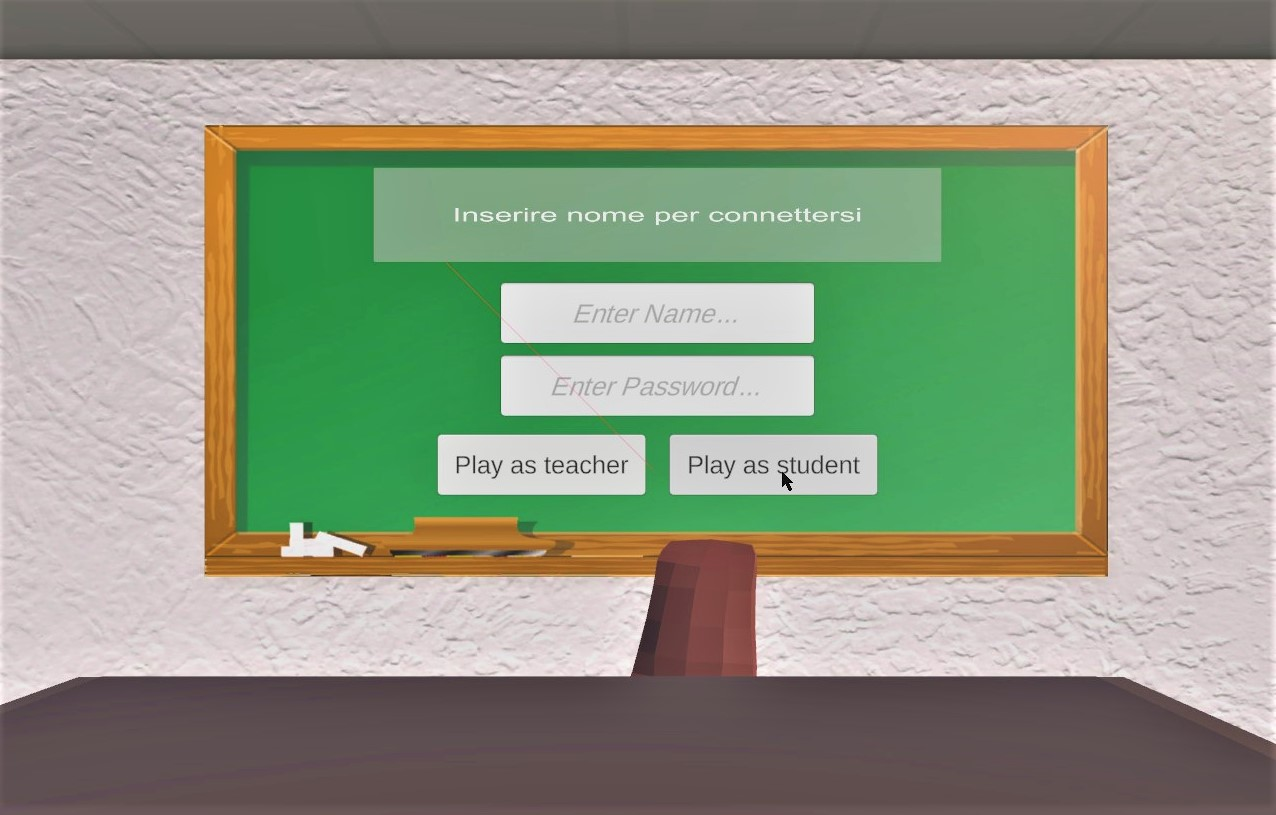
\includegraphics[scale = 0.3]{Immagini/Dimostrazioni d'uso/loginstuderr.jpg}
\caption{Schermata di errore per lo studente}
\label{fig:5.1}
\end{figure}
\begin{figure}[H]
\centering
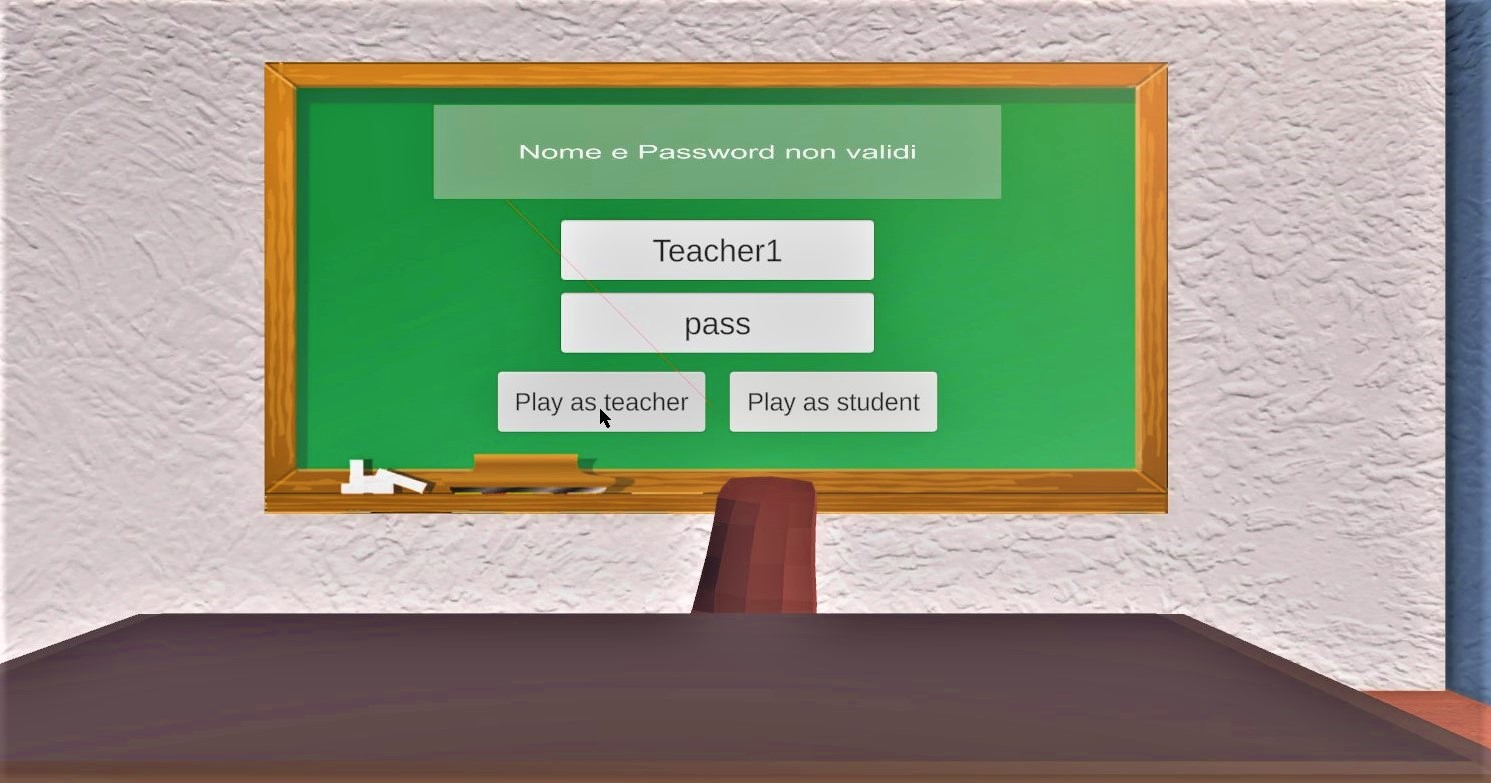
\includegraphics[scale = 0.3]{Immagini/Dimostrazioni d'uso/loginteacherr.jpg}
\caption{Schermata di errore per il docente}
\label{fig:5.2}
\end{figure}
\hspace{-0.6cm}La versione per desktop presenta un problema quando viene eseguita sul visore di riferimento, ovvero l’Oculus Quest 2. 
\\Per delle limitazioni presenti nell'XR Origin, non è possibile utilizzare la tastiera di sistema. 
\\Per ovviare a questo problema, è stato deciso di inserire, nella versione per Oculus Quest 2, un nome di default per gli studenti in modo da poter permettere il login anche tramite visore quando l'utente prova ad accedere senza inserire il nome.
\section{Lobby}
\begin{figure}[H]
\centering
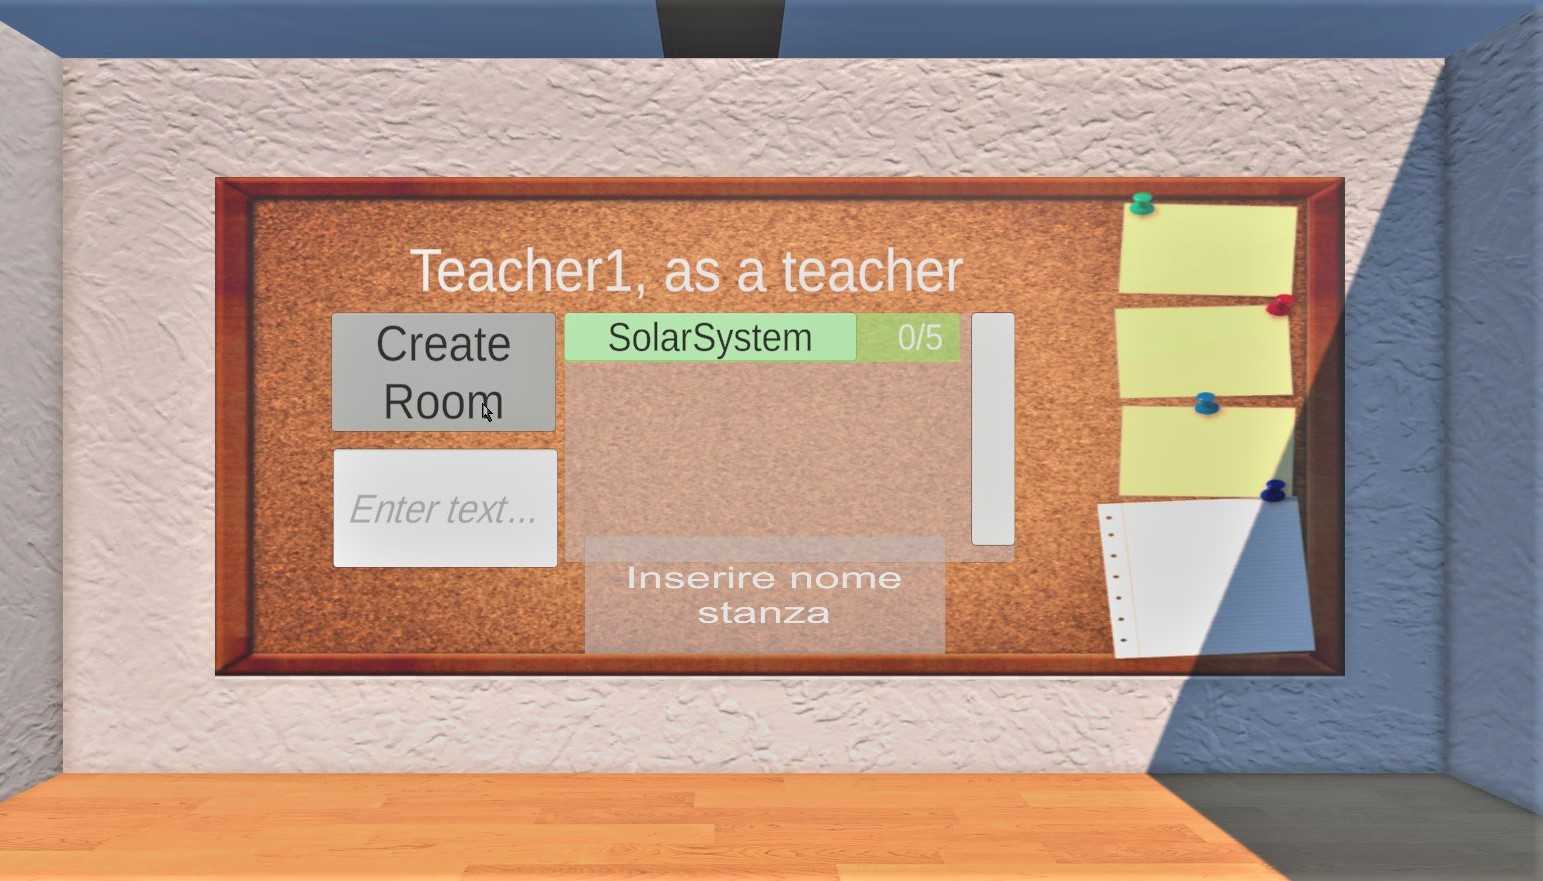
\includegraphics[scale = 0.25]{Immagini/Dimostrazioni d'uso/createroomerr.jpg}
\caption{Lobby docente}
\label{fig:5.3}
\end{figure}
La \textbf{Figura \ref{fig:5.3}} rappresenta la scena che verrà caricata dall'applicazione dell'utente se è stato effettuato l'accesso come docente.
\\Si può notare la presenza del pulsante per creare la stanza (pulsante \textit{Create Room}) e dell'elenco delle stanze disponibili per l'accesso.
\\In particolare, nella figura è presente un messaggio di errore che compare quando il docente cerca di creare una stanza senza nome.
\begin{figure}[H]
\centering
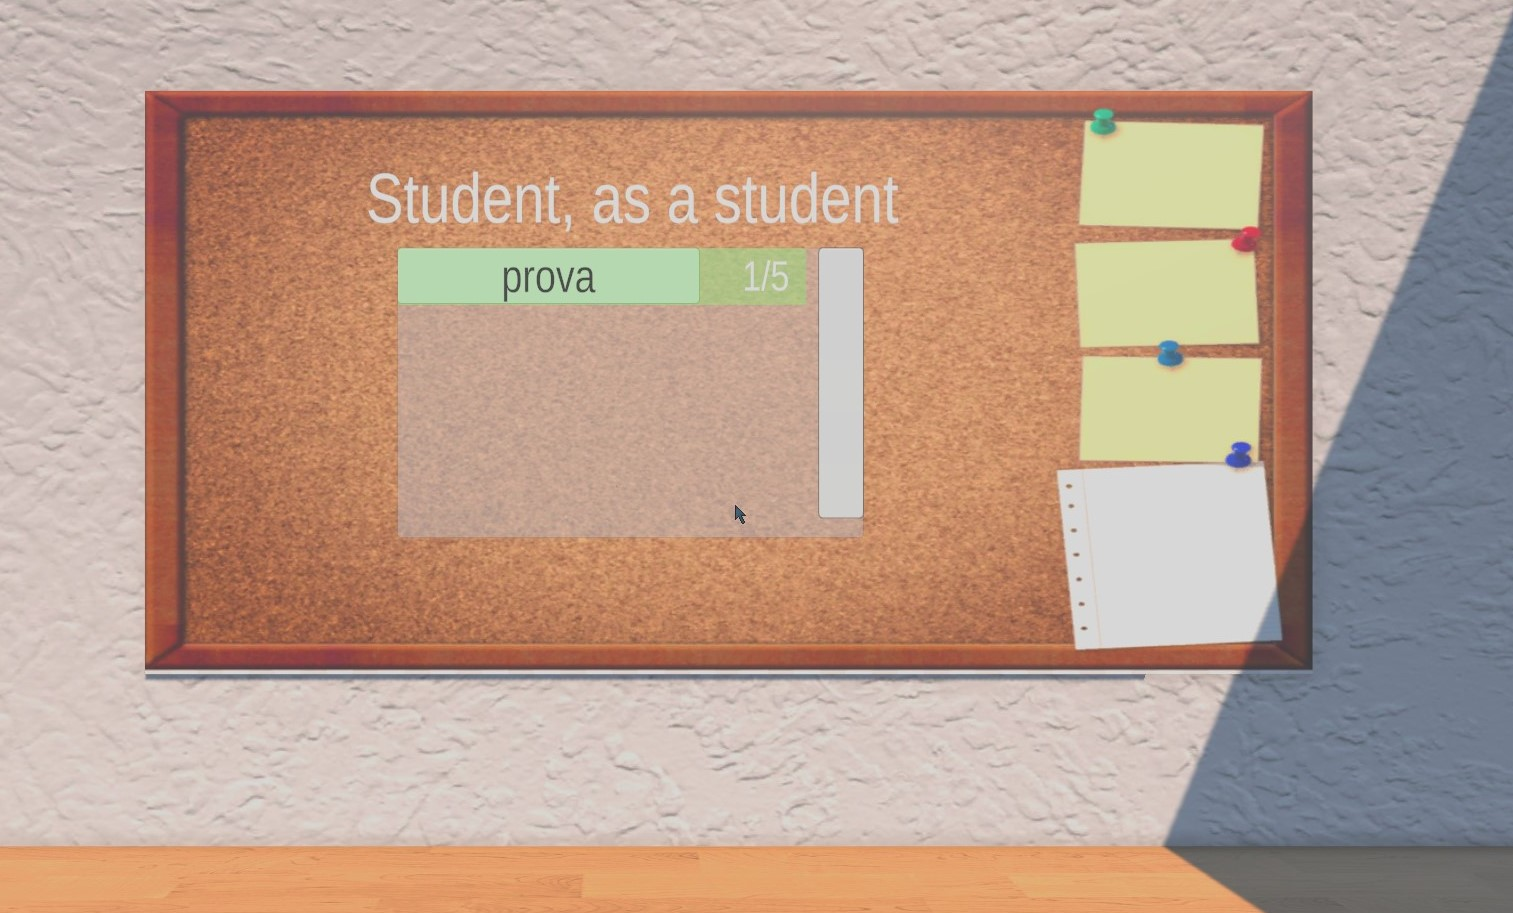
\includegraphics[scale = 0.25]{Immagini/Dimostrazioni d'uso/studlobby.jpg}
\caption{Lobby studente}
\label{fig:5.4}
\end{figure}
\hspace{-0.6cm}La scena rappresentata nella \textbf{Figura \ref{fig:5.4}} è quella caricata dall'applicazione dell'utente se è stato effettuato l'accesso come studente.
\\Lo studente, come già detto nelle specifiche e nei casi d'uso, visualizzerà solo l'elenco delle stanze a cui può unirsi.
\section{Generic Room}
La \textbf{Generic Room} rappresenta la scena del prototipo adibita all'interazione fra gli utenti, ovvero la parte del progetto dove sono implementate le funzionalità descritte nel \textbf{Cap.4}.
\begin{figure}[H]
\centering
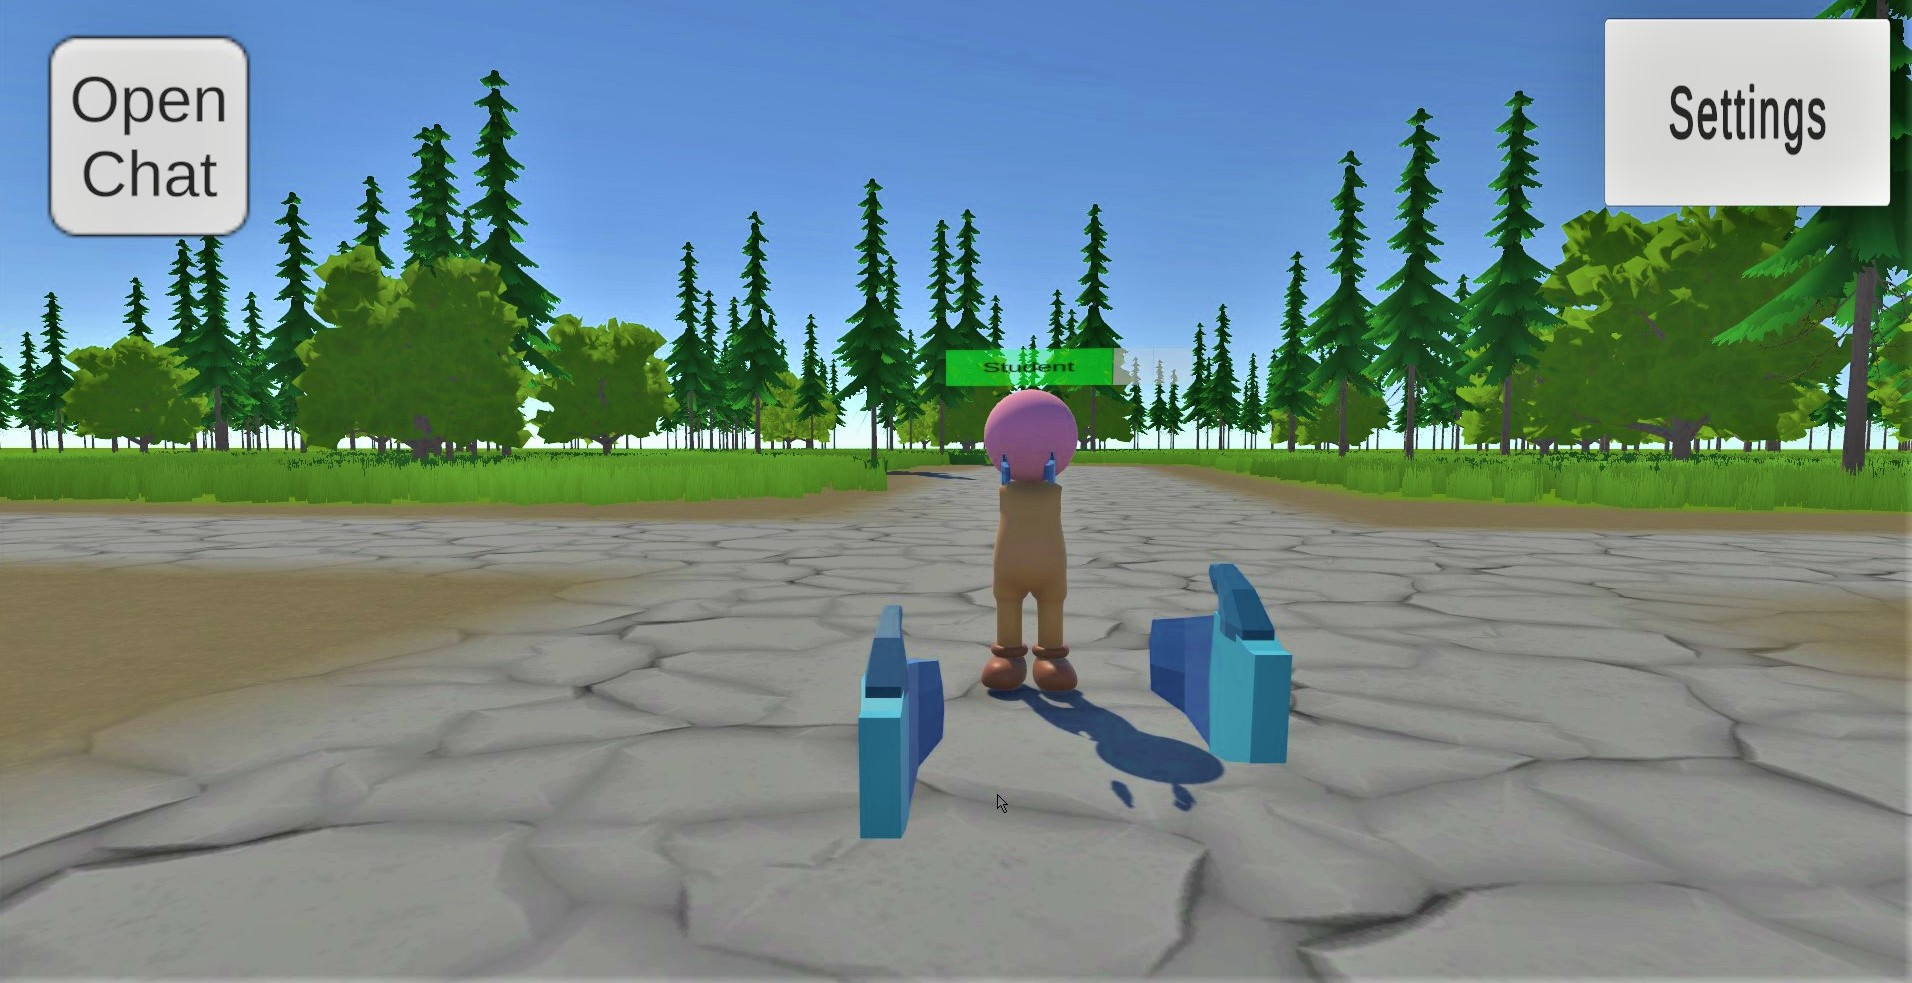
\includegraphics[scale = 0.25]{Immagini/Dimostrazioni d'uso/civediamo.jpg}
\caption{Visualizzazione fra utenti}
\label{fig:5.5}
\end{figure}
\hspace{-0.6cm}Uno dei requisiti fondamentali illustrato nelle specifiche del prototipo è quello della percezione fra utenti.
\\La \textbf{Figura \ref{fig:5.5}} rappresenta la visuale di un utente (\textit{Teacher}), nella quale è ben visibile un secondo utente (\textit{Student}).
\subsection{Chat di testo e Impostazioni}
\begin{figure}[H]
\centering
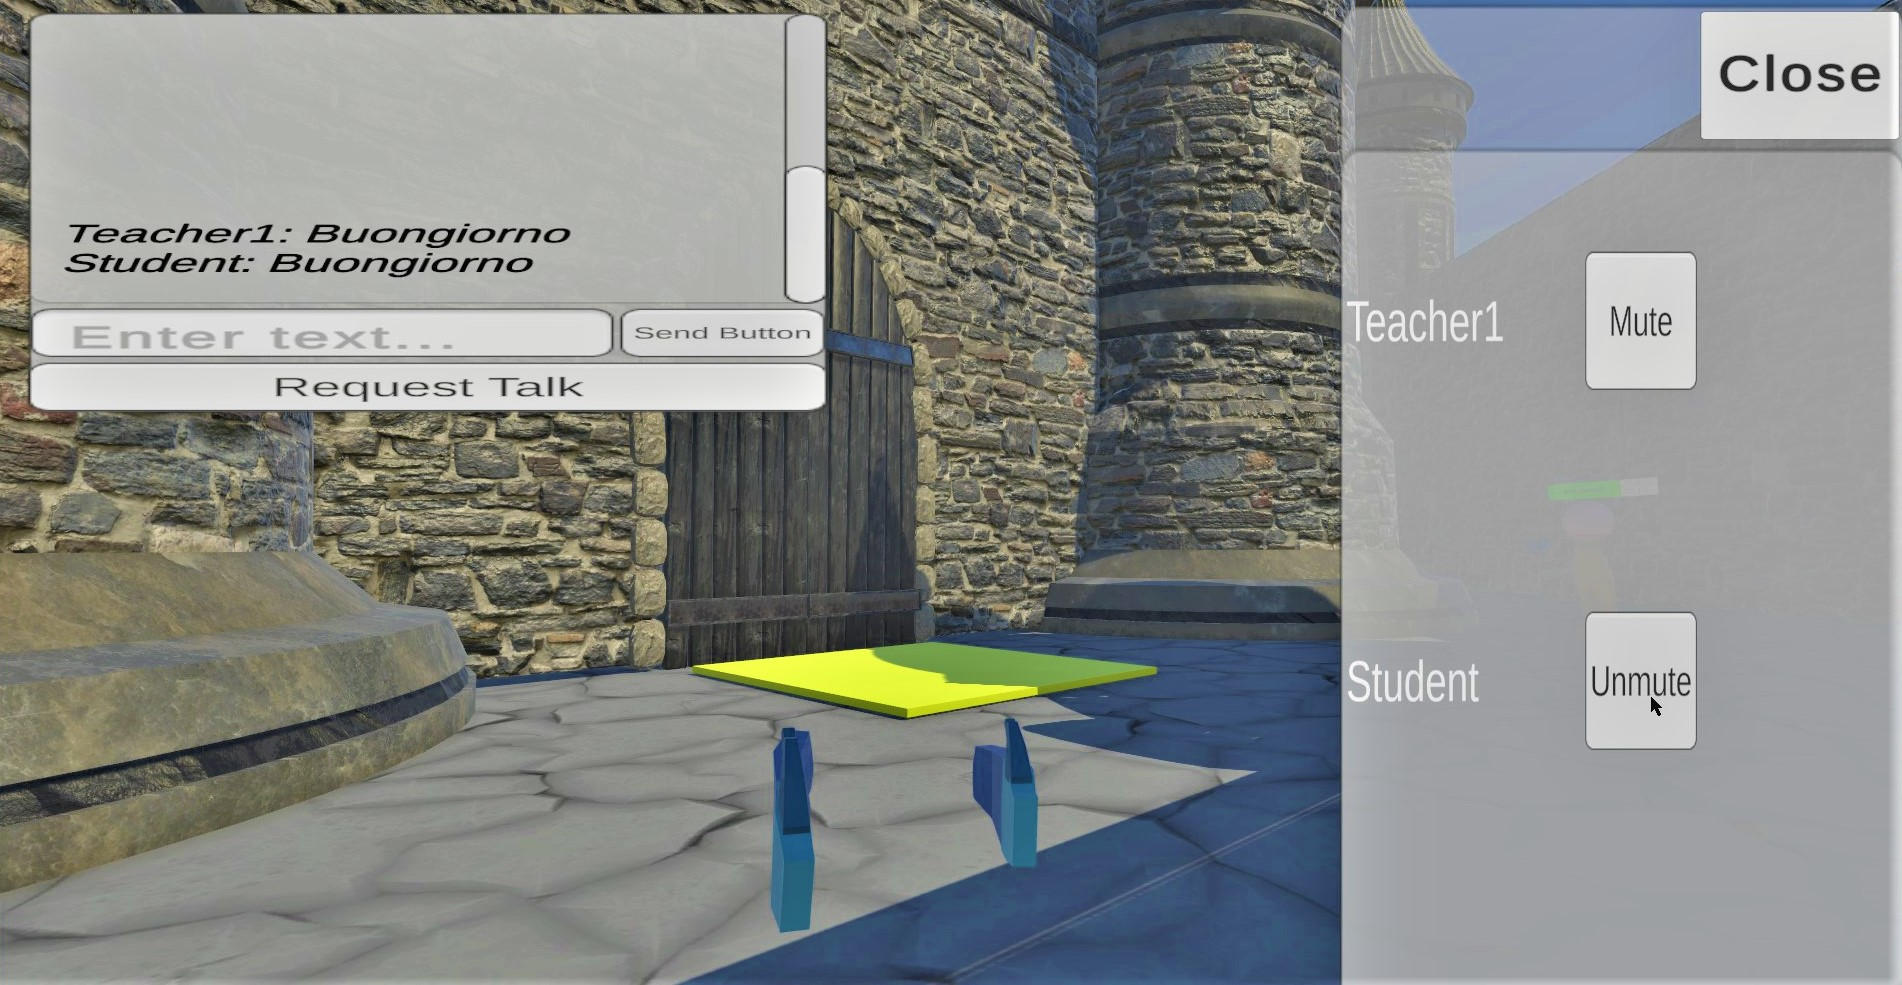
\includegraphics[scale = 0.25]{Immagini/Dimostrazioni d'uso/impostazioni.jpg}
\caption{Funzionamento della Chat e delle Impostazioni}
\label{fig:5.6}
\end{figure}
Nella \textbf{Figura \ref{fig:5.6}} si può notare la presenza della chat sul lato sinistro in cui sono presenti due messaggi, uno inviato dal docente (\textit{Teacher 1}) e uno inviato dallo studente (\textit{Student}).
\\Le impostazioni, che sono accessibili solamente dal docente, si trovano sul lato destro della schermata e, come previsto dai requisti, presentano una lista con i giocatori connessi alla stanza e un bottone per ogni giocatore per l'attivazione o disattivazione del microfono.
\\In particolare, nella figura si nota che il docente ha disattivato il microfono dello studente.
\\La scritta sul bottone accanto al nome dello studente è passata da `Mute` (disattiva il microfono) a `Unmute` (attiva il microfono), se il bottone verrà premuto dal docente, il microfono verrà di nuovo attivato.
\subsection{Creazione/Eliminazione di bandierine}
Le immagini che seguiranno hanno scopo di mostrare sequenzialmente il funzionamento della creazione e distruzione delle bandierine da parte del docente.
\\Saranno presenti immagini sia dal punto di vista del docente sia da quello dello studente, per mostrare in modo ottimale lo svolgimento delle funzionalità.
\\La presenza della chat, nelle suddette immagini, risulta utile per percepire la contemporaneità degli eventi mostrati, infatti sia dal punto di vista dello studente che da quello del docente sono presenti gli stessi messaggi.
\begin{figure}[H]
\centering
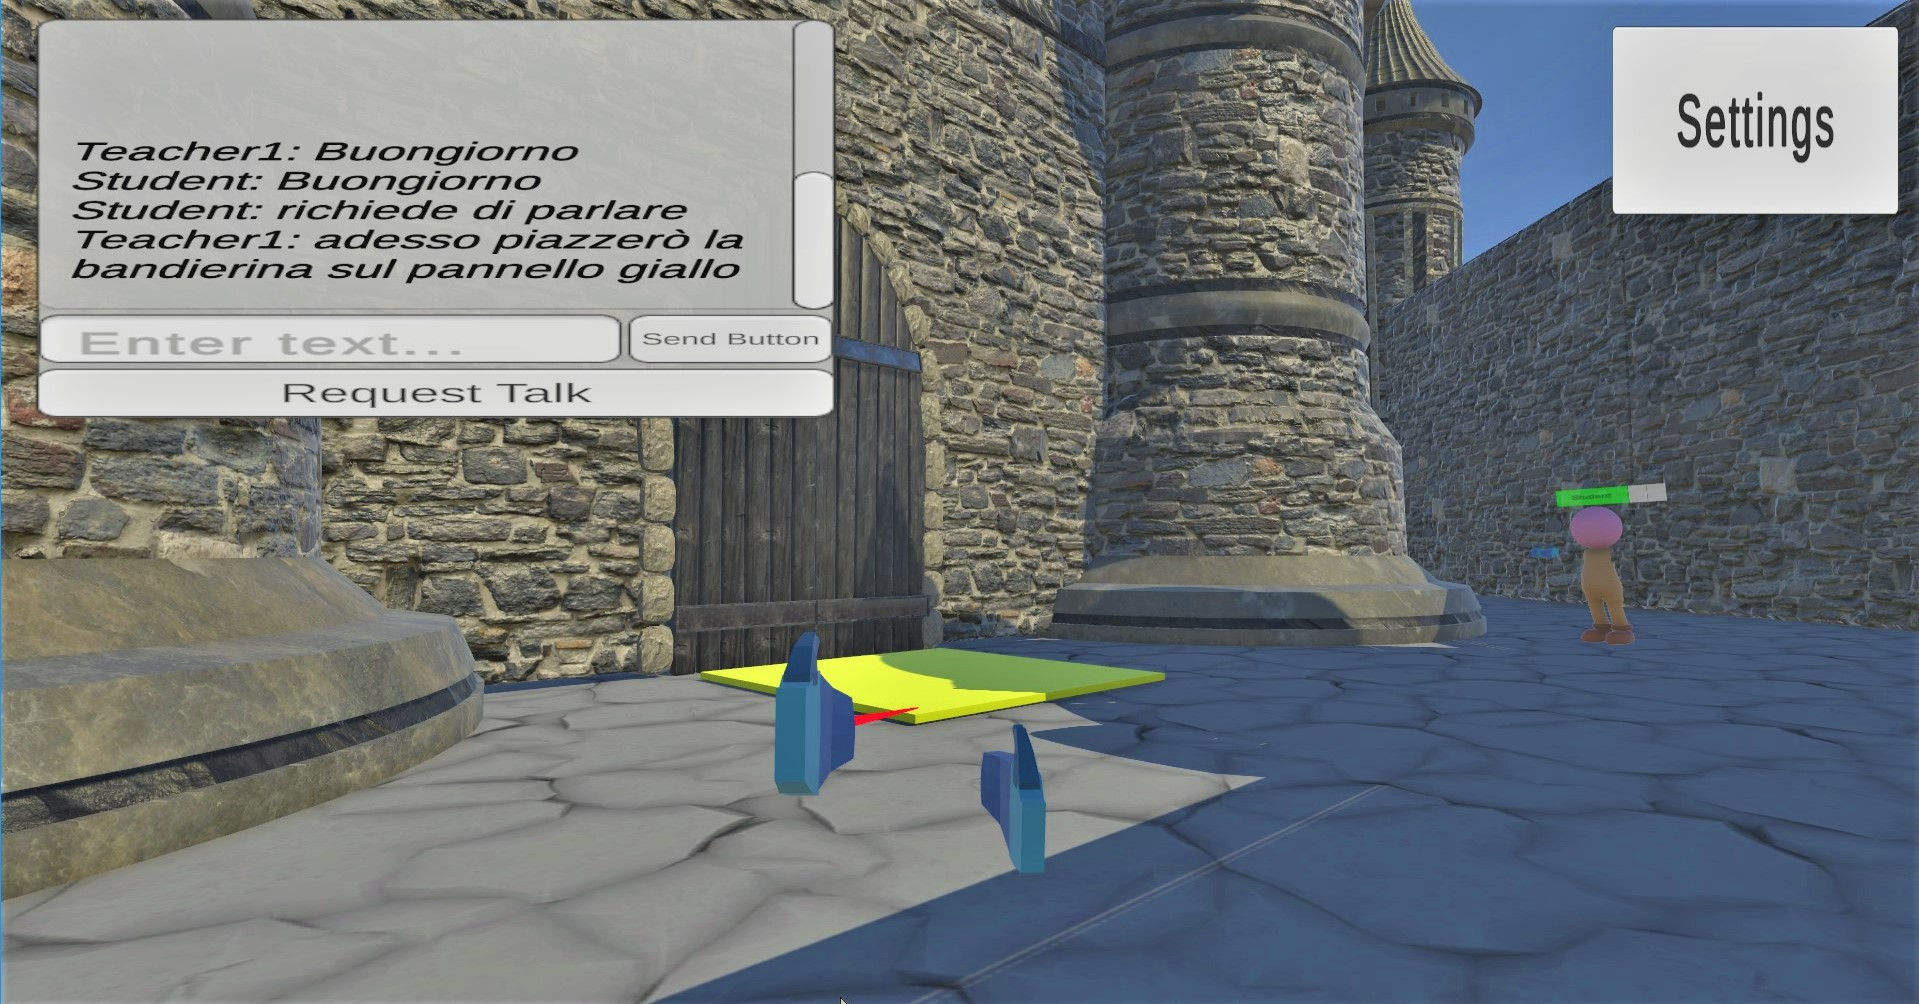
\includegraphics[scale = 0.25]{Immagini/Dimostrazioni d'uso/piazzobandierina.jpg}
\caption{Scena prima del piazzamento della bandierina}
\end{figure}
\begin{figure}[H]
\centering
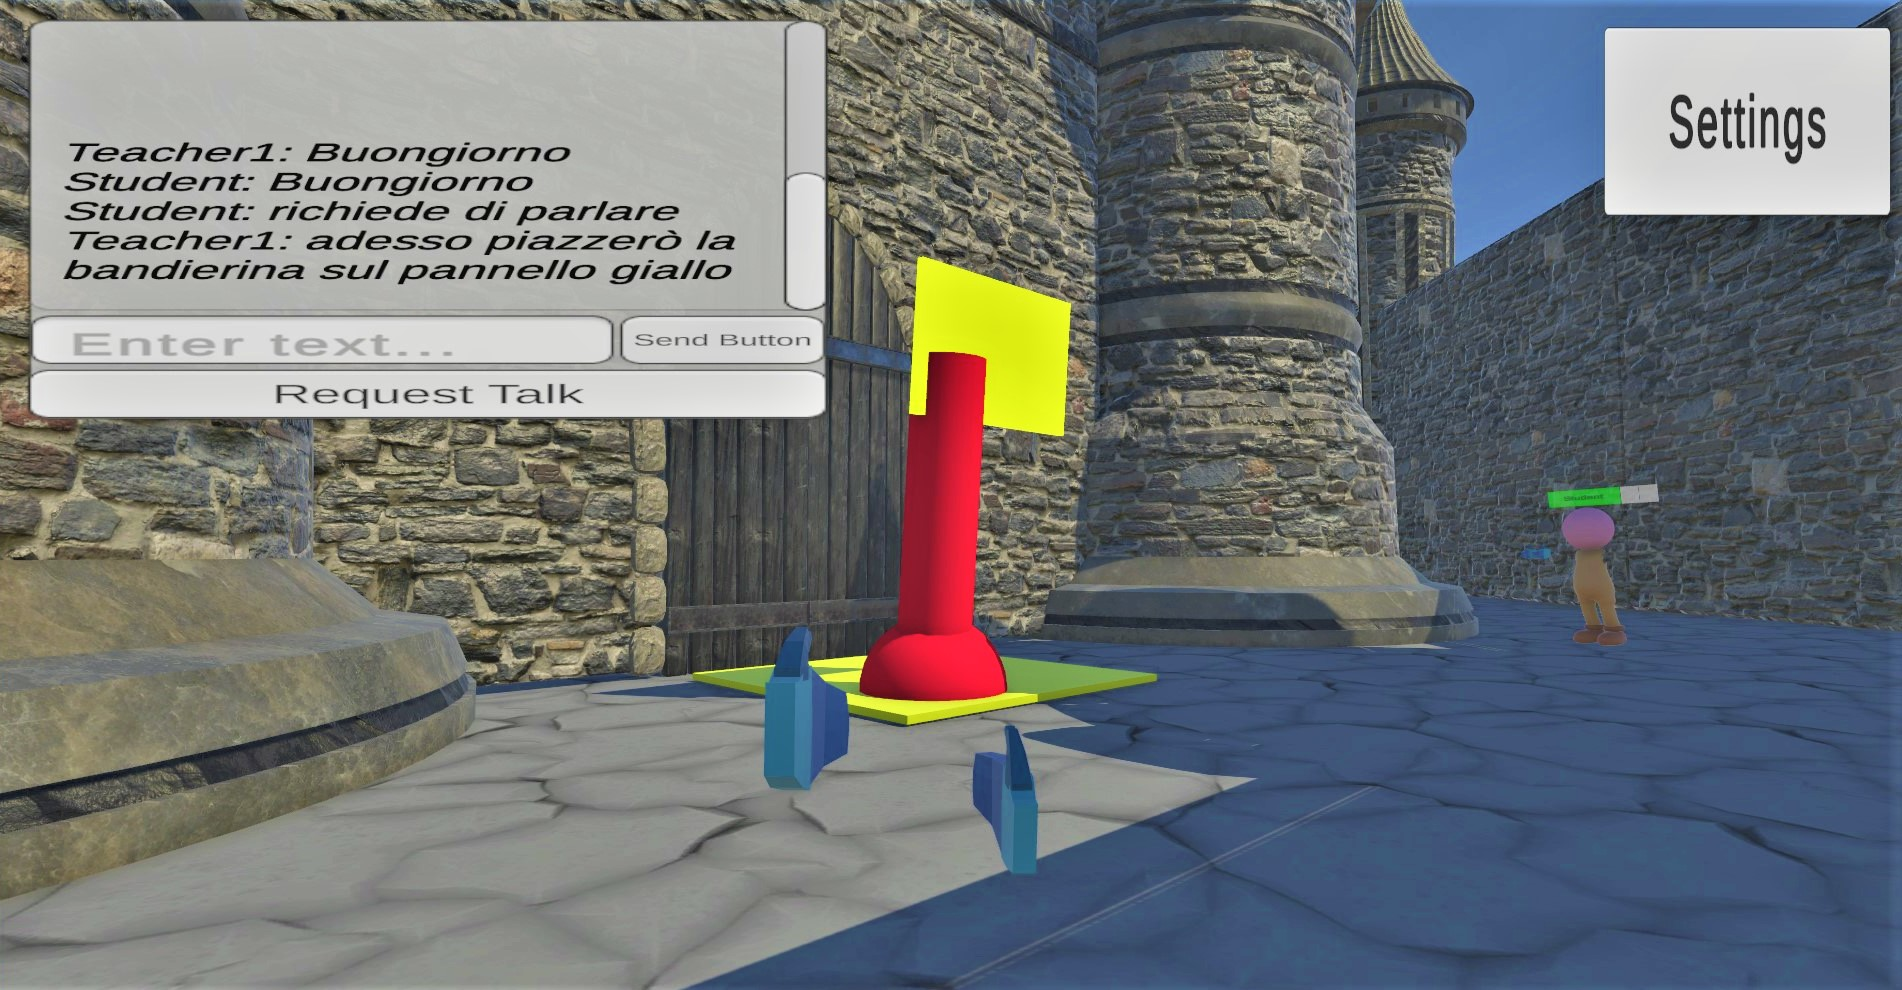
\includegraphics[scale = 0.25]{Immagini/Dimostrazioni d'uso/bandierinapiazzatalatodocente.jpg}
\caption{Scena dopo il piazzamento della bandierina lato docente}
\end{figure}\begin{figure}[H]
\centering
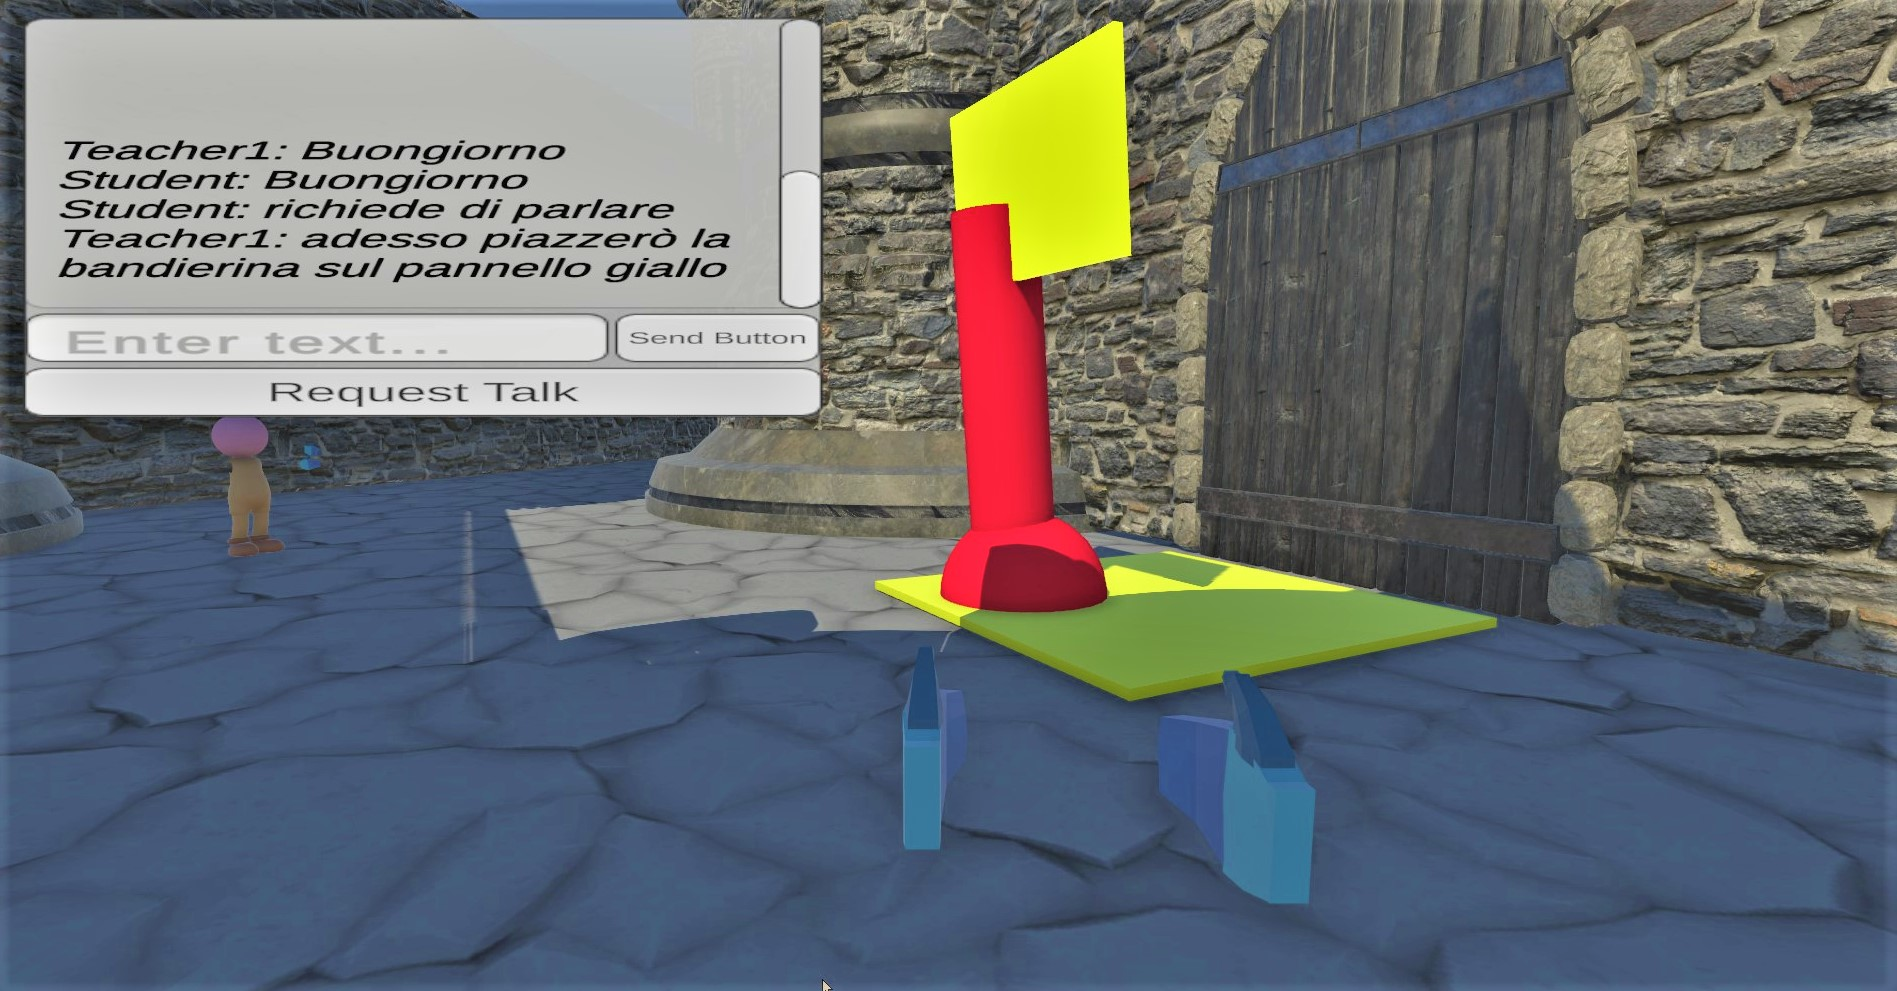
\includegraphics[scale = 0.25]{Immagini/Dimostrazioni d'uso/bandierinapiazzatalatostudente.jpg}
\caption{Scena dopo il piazzamento della bandierina lato studente}
\end{figure}
\begin{figure}[H]
\centering
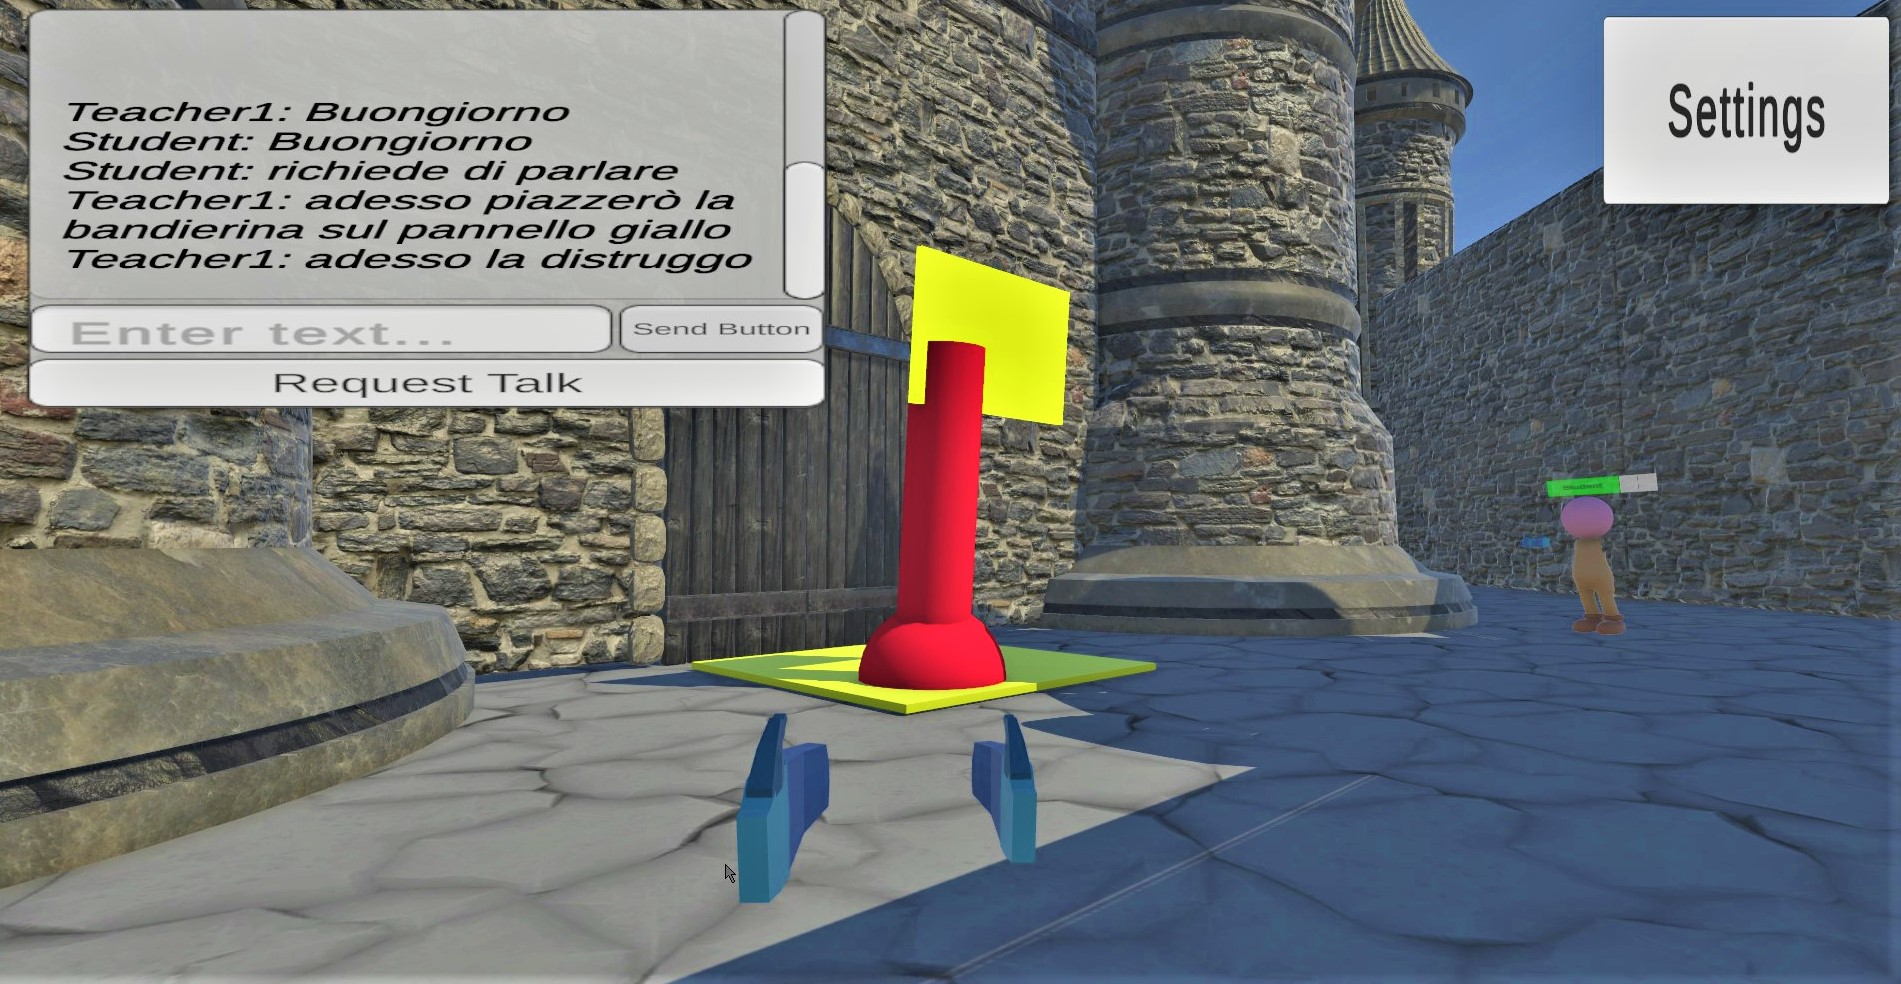
\includegraphics[scale = 0.25]{Immagini/Dimostrazioni d'uso/adessoladistruggo.jpg}
\caption{Scena prima della distruzione della bandierina}
\end{figure}
\begin{figure}[H]
\centering
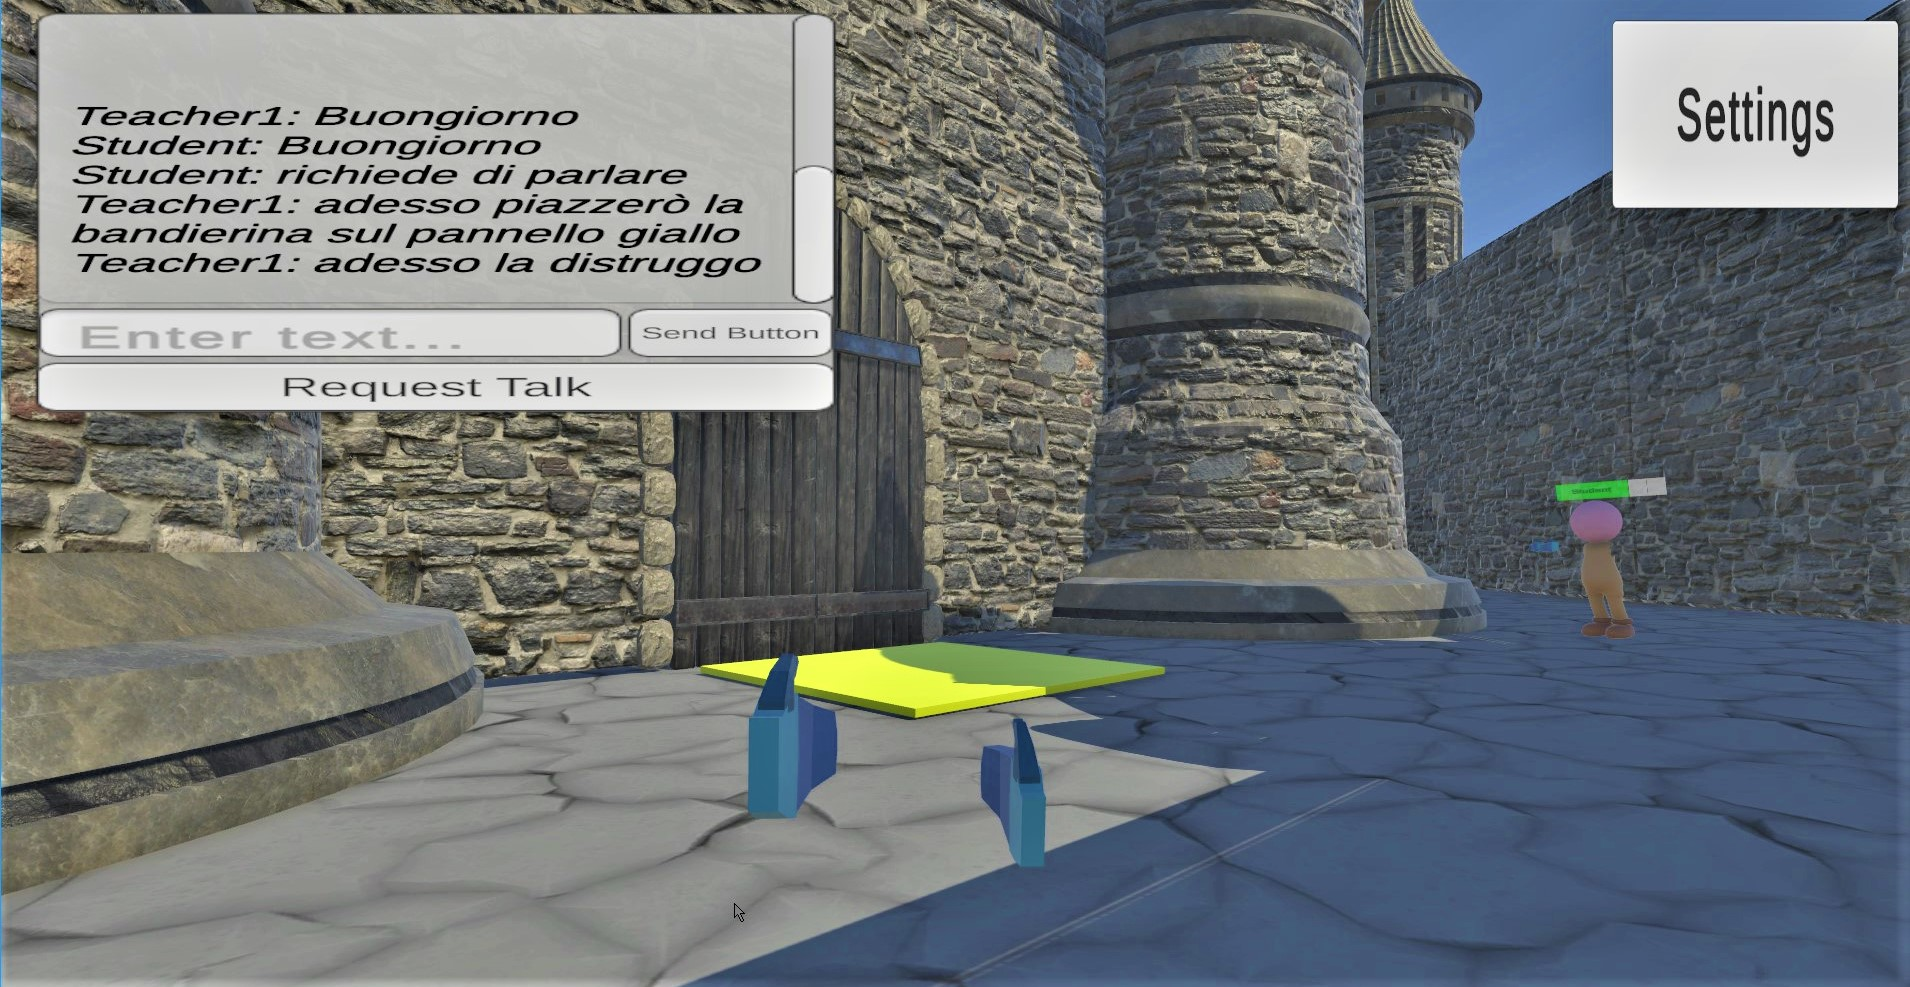
\includegraphics[scale = 0.25]{Immagini/Dimostrazioni d'uso/bandierinadistruttalatodoc.jpg}
\caption{Scena dopo la distruzione della bandierina lato docente}
\end{figure}
\begin{figure}[H]
\centering
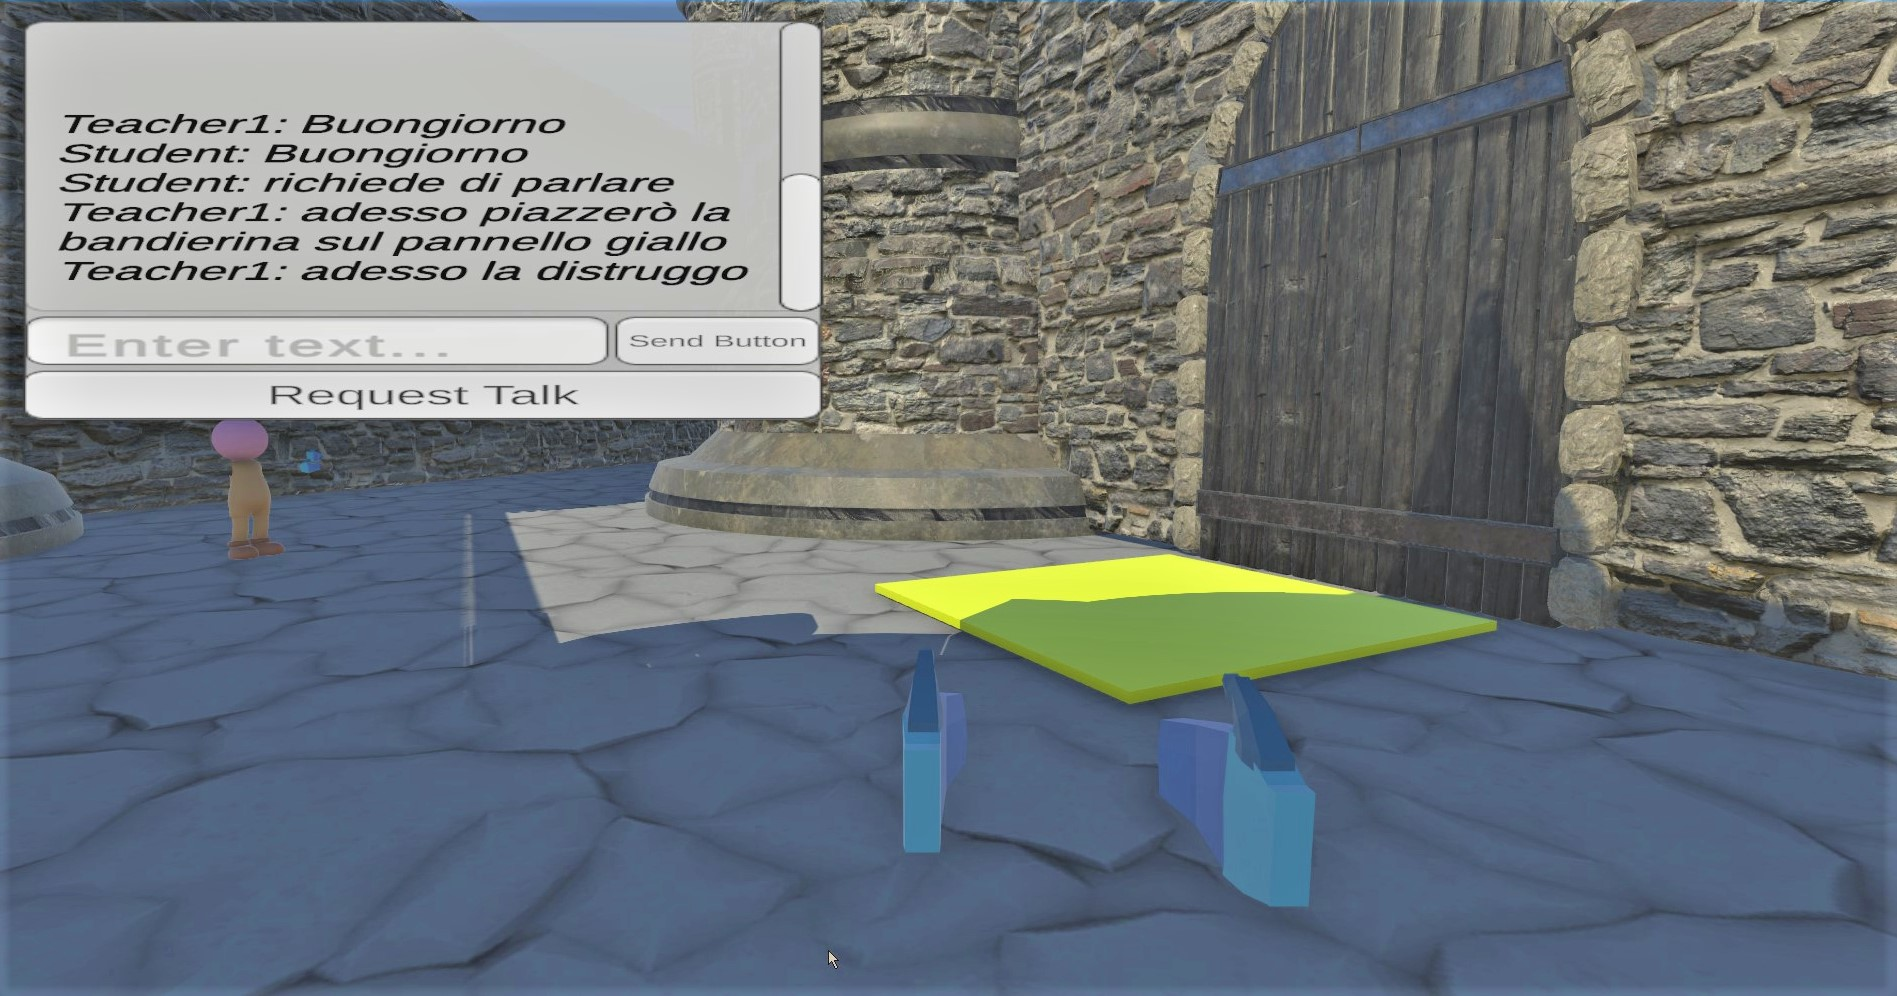
\includegraphics[scale = 0.25]{Immagini/Dimostrazioni d'uso/bandierinadistruttalatostud.jpg}
\caption{Scena dopo la distruzione della bandierina lato studente}
\end{figure}